\documentclass[tikz]{standalone}

\usepackage{tikz}
\usetikzlibrary{automata}

\begin{document}

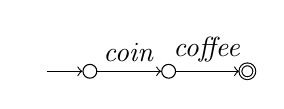
\begin{tikzpicture}
    \tikzstyle{every state}=[
        draw,
        shape=circle,
        inner sep=1pt,
        minimum size=5pt,
        final/.style={double,minimum size=6pt},
        initial text=]

    [auto,->]
    \renewcommand{\a}[1]{\textit{#1}}
    \node[state,initial] (n0) {}; 
    \node[state, right of=n0] (n1) {}; 
    \node[state, accepting, right of=n1] (n2) {};
    \path[->] (n0) edge node[above]{\a{coin}} (n1) (n1) edge node[above]{\a{coffee}} (n2);
\end{tikzpicture}
\end{document}